% !TeX root = ex2.tex
\subsection{Video and Images}

\subsubsection*{Video to images}

Download video from \href{https://github.com/opencv/opencv/blob/master/samples/data/vtest.avi}{here} and store as \texttt{./videos/vtest.avi}. Then run the following

\begin{verbatim}
    python .\vid_to_imgs.py -n 10
\end{verbatim}

The code is shown in listing \ref{lst:q2-vid-to-imgs}. Output is in figure \ref{fig:q2-v2i-seq}.

\lstinputlisting[language=python, caption={vid\_to\_imgs.py}, label=lst:q2-vid-to-imgs]{../python/vid_to_imgs.py}

The above script (listing \ref{lst:q2-vid-to-imgs}) gives the following output (along with a GUI window to show the images of the video)

\begin{verbatim}
    Folder ./out is being created
    Reached 10 frames
    Wrote 10 frames under ./out/img*.jpg
\end{verbatim}

\begin{figure}[t]
    \centering
    \begin{subfigure}[b]{0.3\textwidth}
        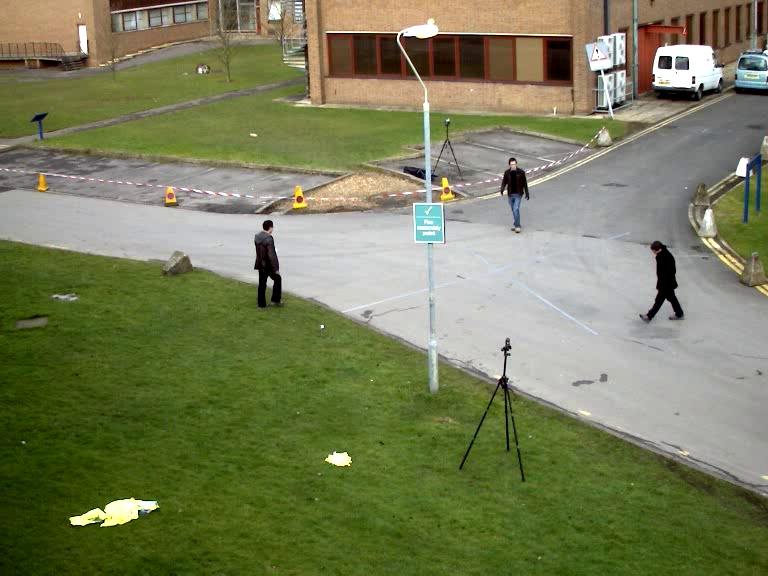
\includegraphics[width=\textwidth]{../out/img1.jpg}
        \caption{Image 1}
    \end{subfigure}
    \begin{subfigure}[b]{0.3\textwidth}
        \includegraphics[width=\textwidth]{../out/img5.jpg}
        \caption{Image 5}
    \end{subfigure}
    \begin{subfigure}[b]{0.3\textwidth}
        \includegraphics[width=\textwidth]{../out/img10.jpg}
        \caption{Image 10}
    \end{subfigure}
    \caption{Sequence of images}
    \label{fig:q2-v2i-seq}
    \small
        First, fifth, and tenth image in the 10-image sequence produced by listing \ref{lst:q2-vid-to-imgs}.
\end{figure}

Learned the following things in this question

\begin{itemize}
    \item Using \href{https://docs.python.org/3.10/library/argparse.html}{argparse} module to parse arguments passed to a script
    \item Reading a video file (reference from \href{https://docs.opencv.org/4.x/dd/d43/tutorial_py_video_display.html}{tutorial})
\end{itemize}
